\section{Resultados y análisis}


\subsection{Verificación de los valores del giroscopio, batería y USART en la pantalla LCD}

Se realizaron pruebas por separado para poder verificar el correcto funcionamiento del giroscopio, de la batería y del USART.

\subsubsection{Verificación de la lectura del giroscopio}

    \begin{figure}[H]
        \begin{subfigure}{0.5\textwidth}
        \centering
        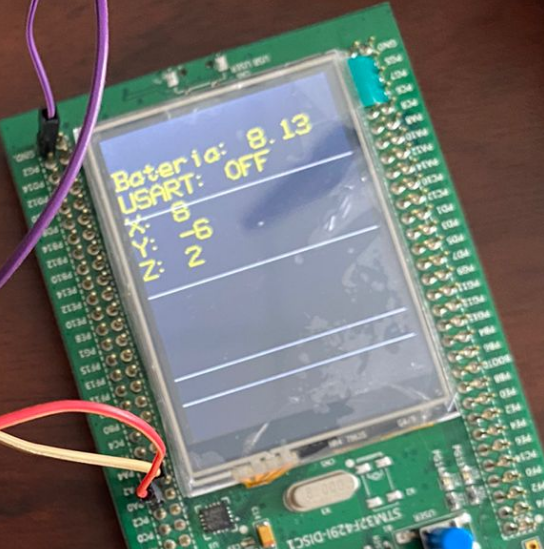
\includegraphics[width=\textwidth]{Imagenes/giroscopio2.png} 
        \caption{Prueba del giroscopio sobre la mesa sin movimiento.}
        \label{Fig:giroscopio}
    \end{subfigure}
    \begin{subfigure}{0.5\textwidth}
        \centering
        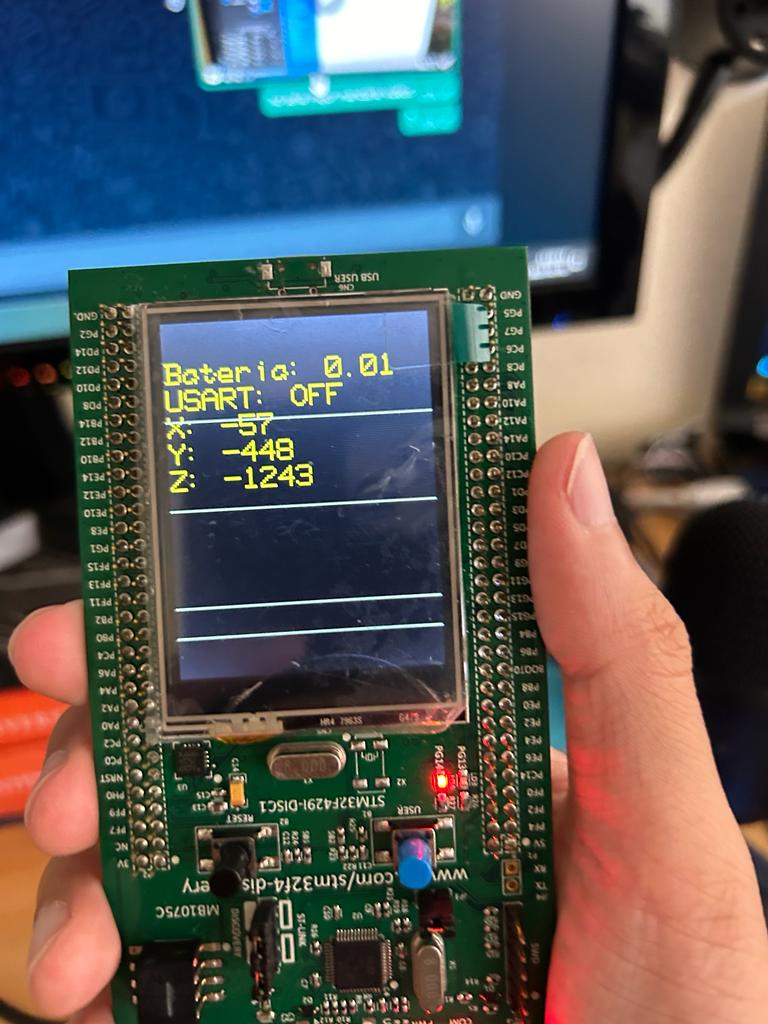
\includegraphics[width=\textwidth]{Imagenes/giroscopio.jpg} 
        \caption{Prueba del giroscopio levantándolo y con movimiento.}
        \label{Fig:giroscopio2}
    \end{subfigure}
    \end{figure}

En la figura \ref{Fig:giroscopio}, se puede observar que esta prueba fue cuando el microcontrolador estaba sobre la mesa, al estar en la mesa los valores que se obtienen son cercanos a 0, no son cero ya que es probable que el giroscopio sea muy sensible ante cualquier movimiento, aunque sea muy pequeño, por esta razón siempre marca algún valor aunque parezca que no esta en movimiento, y en la figura \ref{Fig:giroscopio2} se puede observar cómo la lectura del giroscopio cambia al someterse a un movimiento, en este caso se levantó de la mesa, demostrando así que los valores de \textit{X}, \textit{Y} y \textit{Z} cambian y así poder simular un sismógrafo.
Adicionalmente, en la entrega de este reporte se incluye tres videos, donde cualquiera de los tres videos se observa que se realiza la lectura del giroscopio correctamente.

\subsubsection{Verificación de la lectura de la Batería}

    \begin{figure}[H]
        \begin{subfigure}{0.5\textwidth}
        \centering
        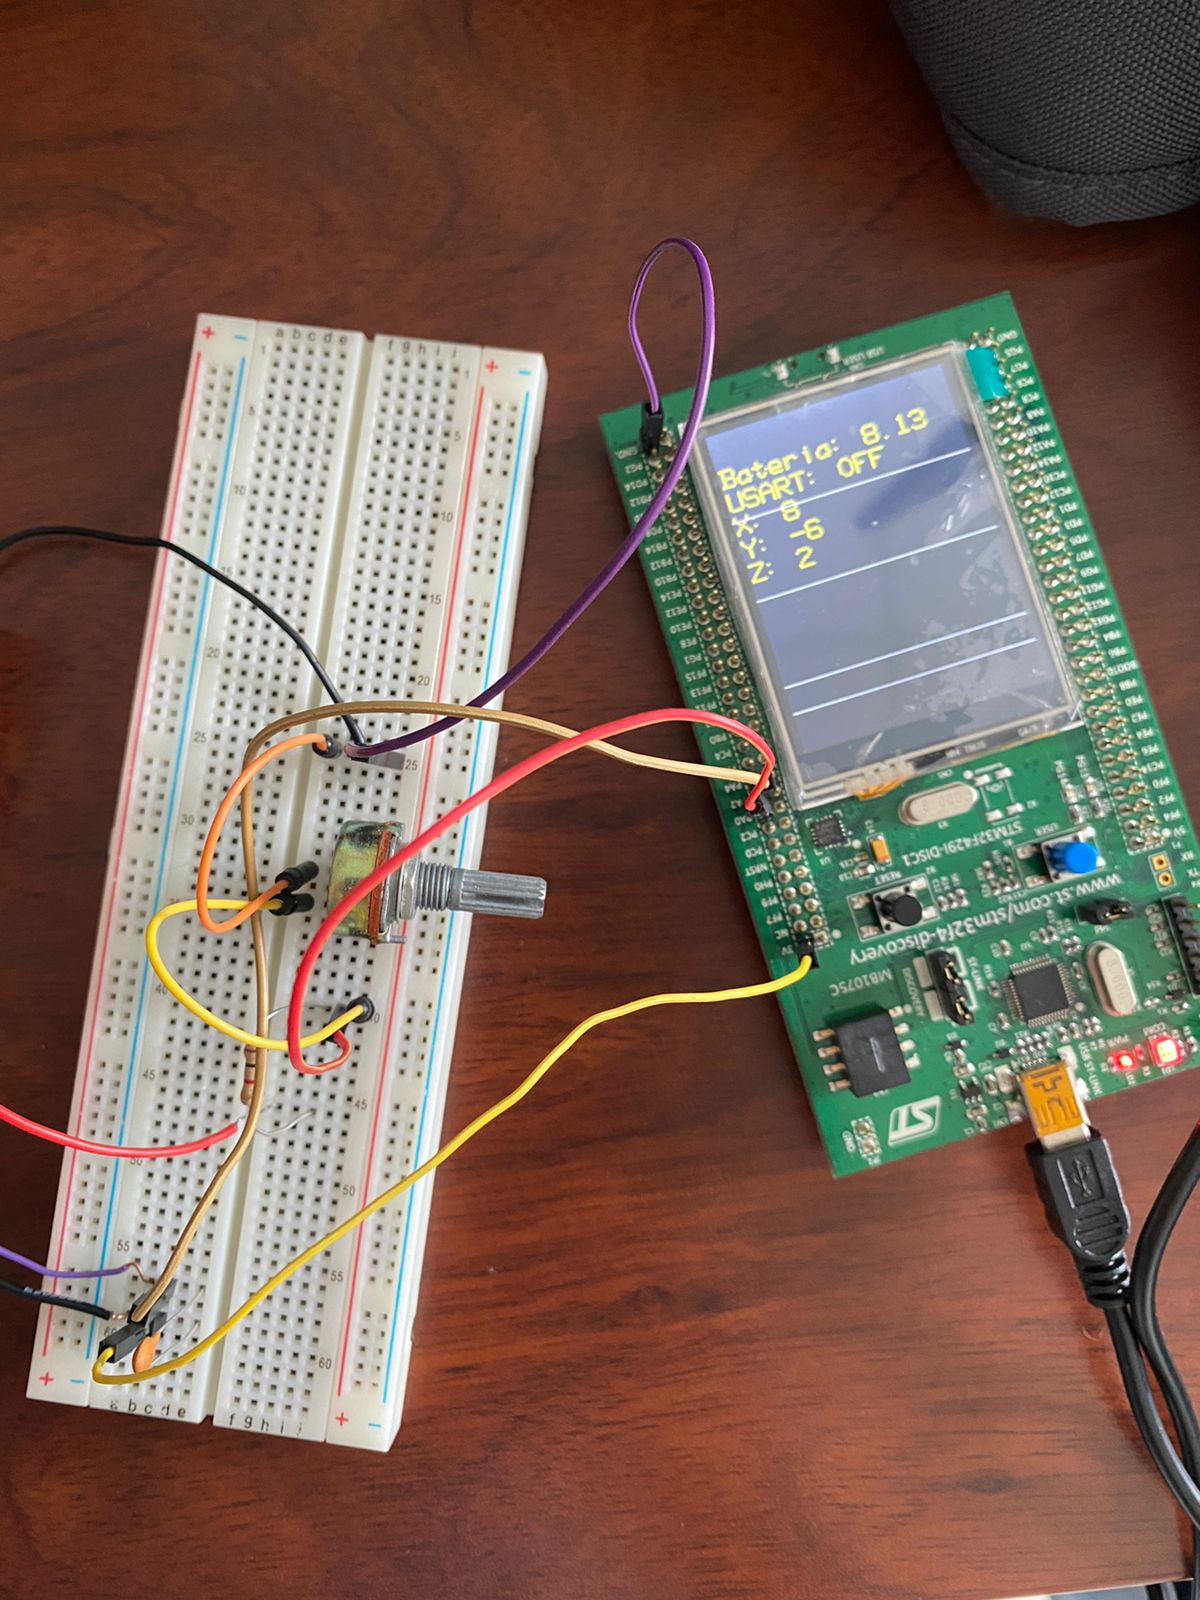
\includegraphics[width=\textwidth]{Imagenes/Prueba_Bat.jpg} 
        \caption{Prueba Batería en rango lejos de 7V.}
        \label{Fig:Prueba_Bat}
    \end{subfigure}
    \begin{subfigure}{0.5\textwidth}
        \centering
        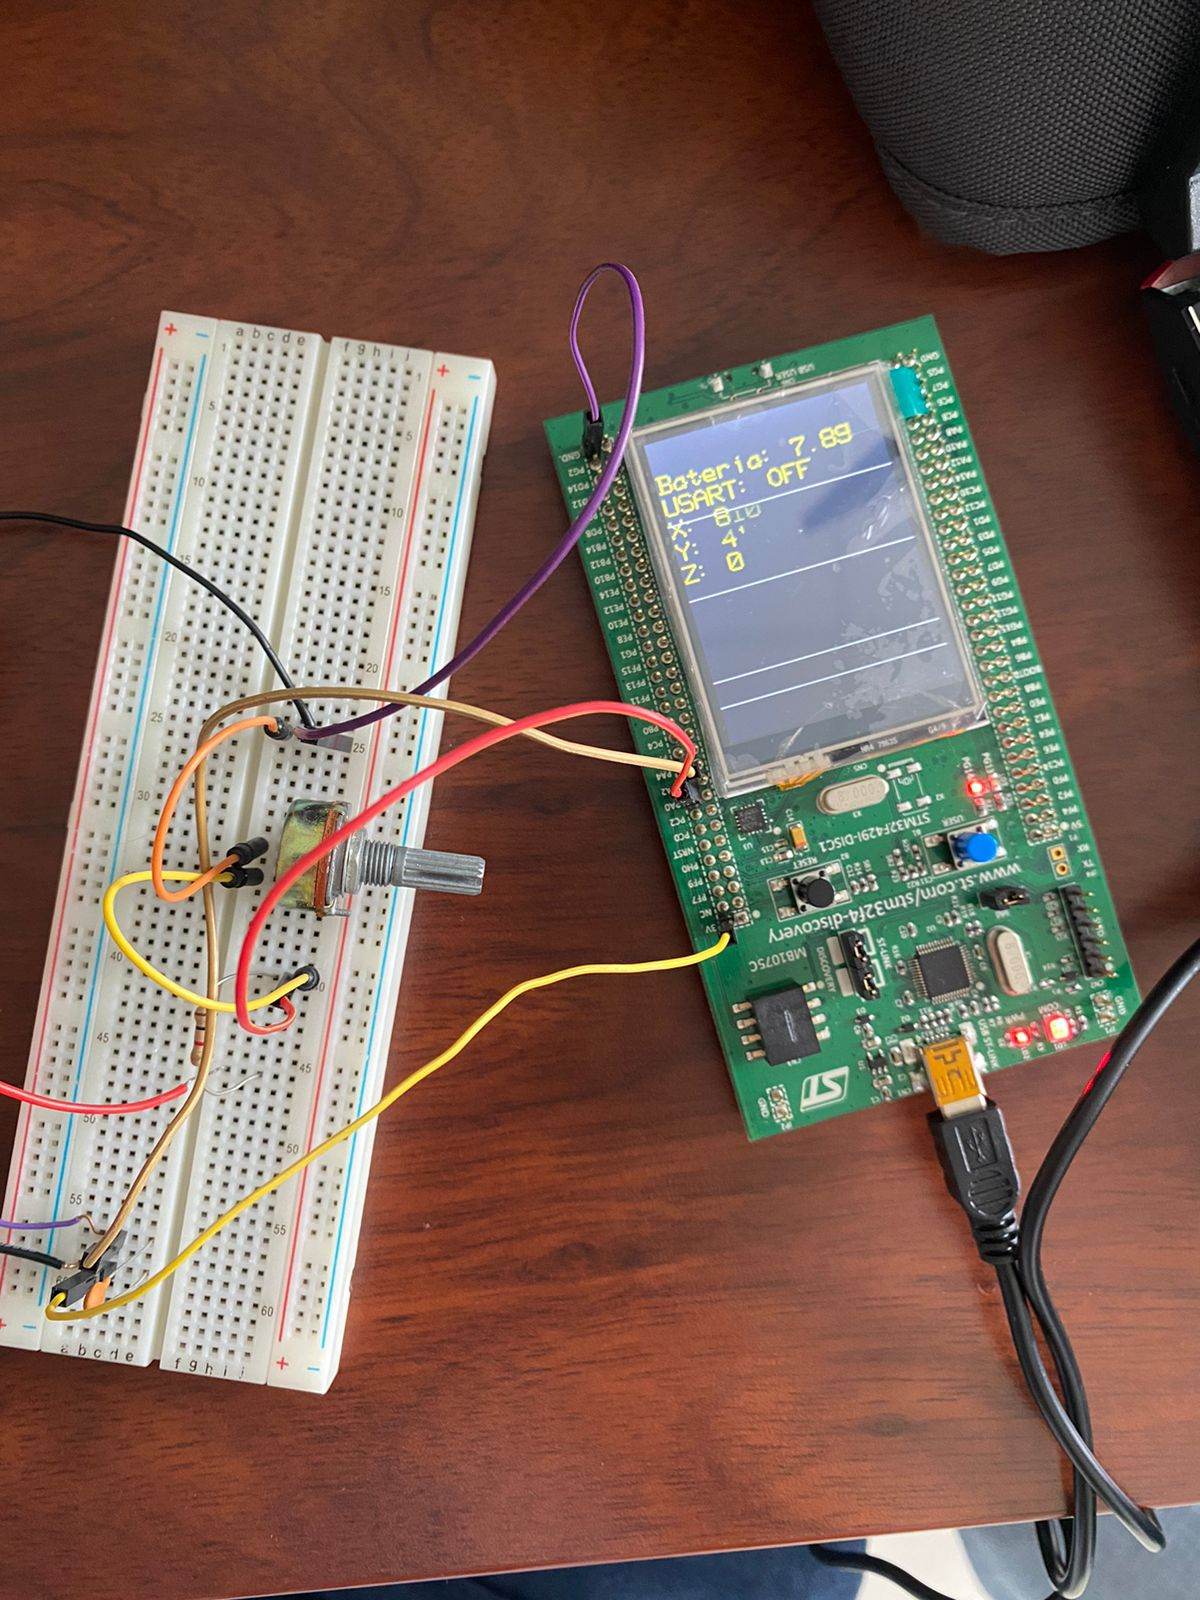
\includegraphics[width=\textwidth]{Imagenes/Prueba_Bat2.jpg} 
        \caption{Prueba Batería en rango cercano a 7V.}
        \label{Fig:Prueba_Bat2}
    \end{subfigure}
    \end{figure}

Como se observan en las figuras \ref{Fig:Prueba_Bat} y \ref{Fig:Prueba_Bat2}, se realizó una configuración de un divisor de tensiones con un potenciómetro con el fin de poder simular una caída de tensión de la batería, y conectando el pin PA0 a la salida de ese circuito y protegiendo así el STM32F429, entonces cuando el microcontrolador lee de la batería 8V o más, el cual se mantiene lejos del limite de operación del microcontrolador, el LED rojo que tiene incorporado el microcontrolador se encuentra apagado. Luego, se ajusta el potenciómetro de manera que lee una tensión por debajo de 8V y cerca a la tensión de operación, entonces el LED rojo se enciende y parpadea, indicando que se está trabajando con una tensión muy cercana a la tensión de operación del STM32F429 como se observa en la figura \ref{Fig:Prueba_Bat2}.


\subsubsection{Verificación de la lectura de la USART}

\begin{figure}[H]
    \begin{subfigure}{0.5\textwidth}
    \centering
    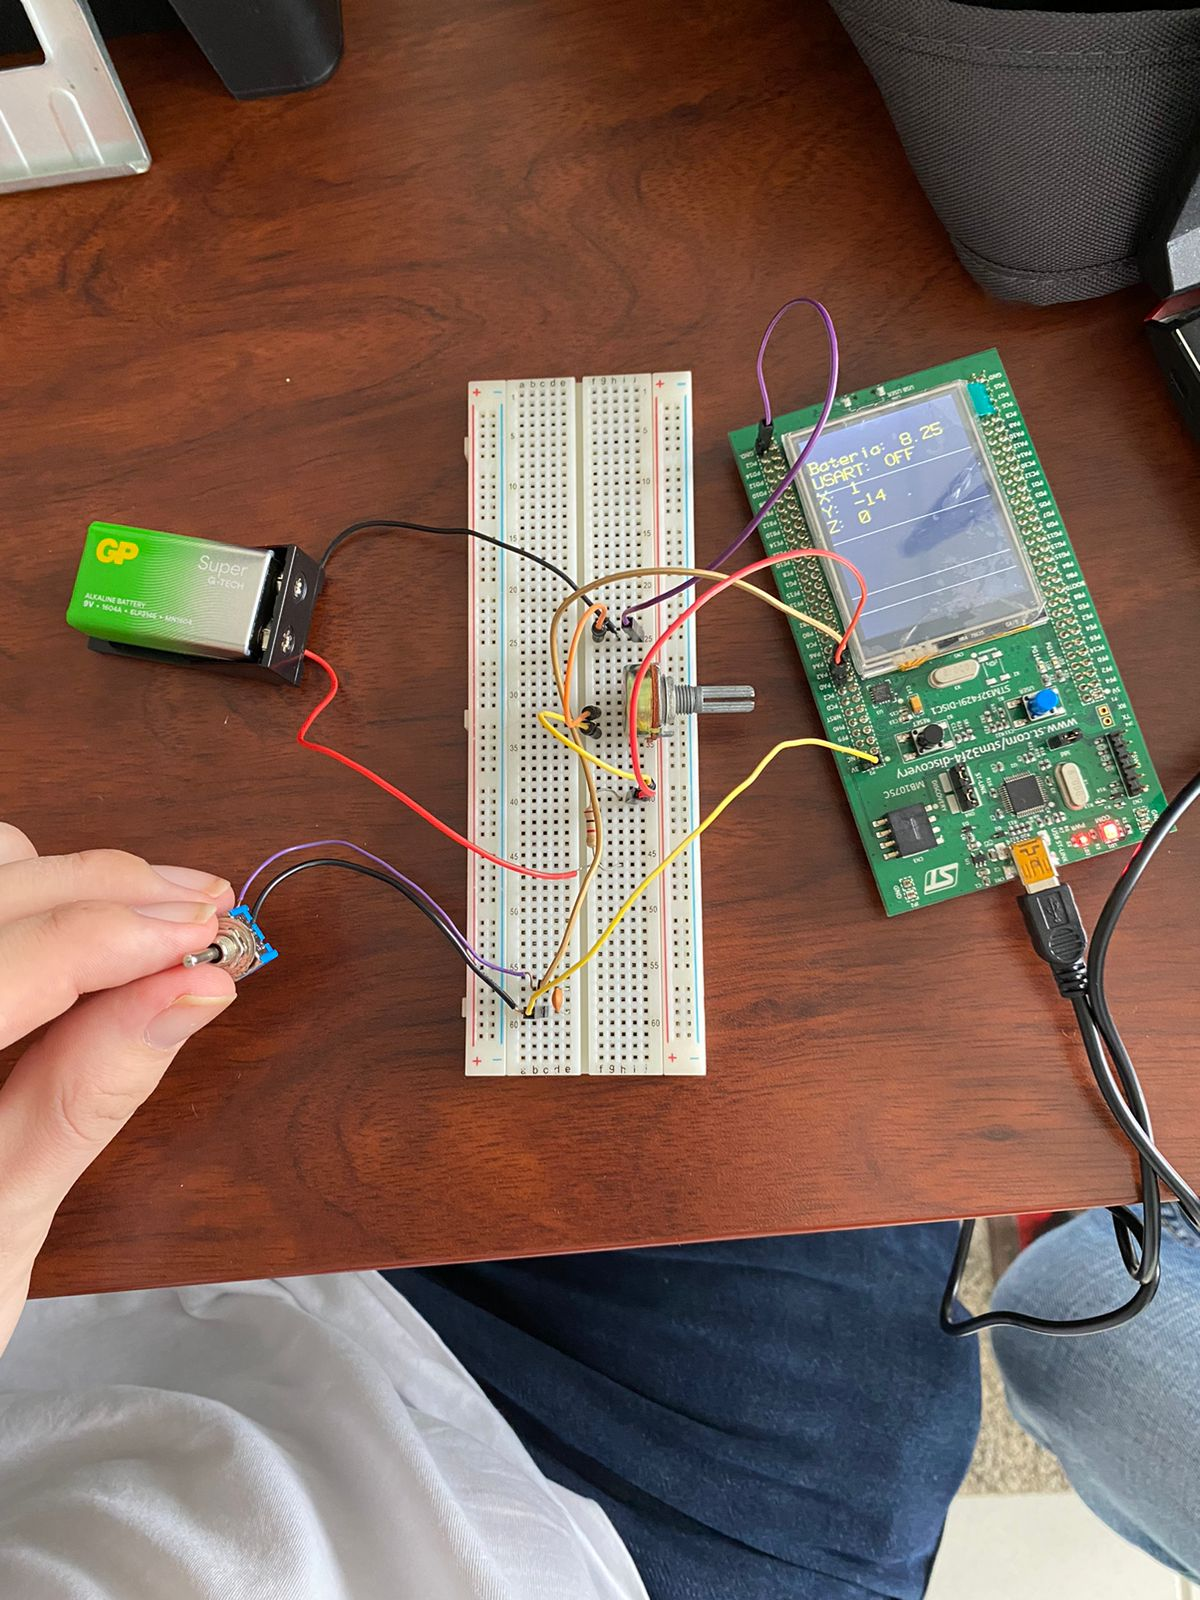
\includegraphics[width=\textwidth]{Imagenes/Prueba_USART.jpg} 
    \caption{Prueba USART en estado ``OFF''}
    \label{Fig:Prueba_USART}
\end{subfigure}
\begin{subfigure}{0.5\textwidth}
    \centering
    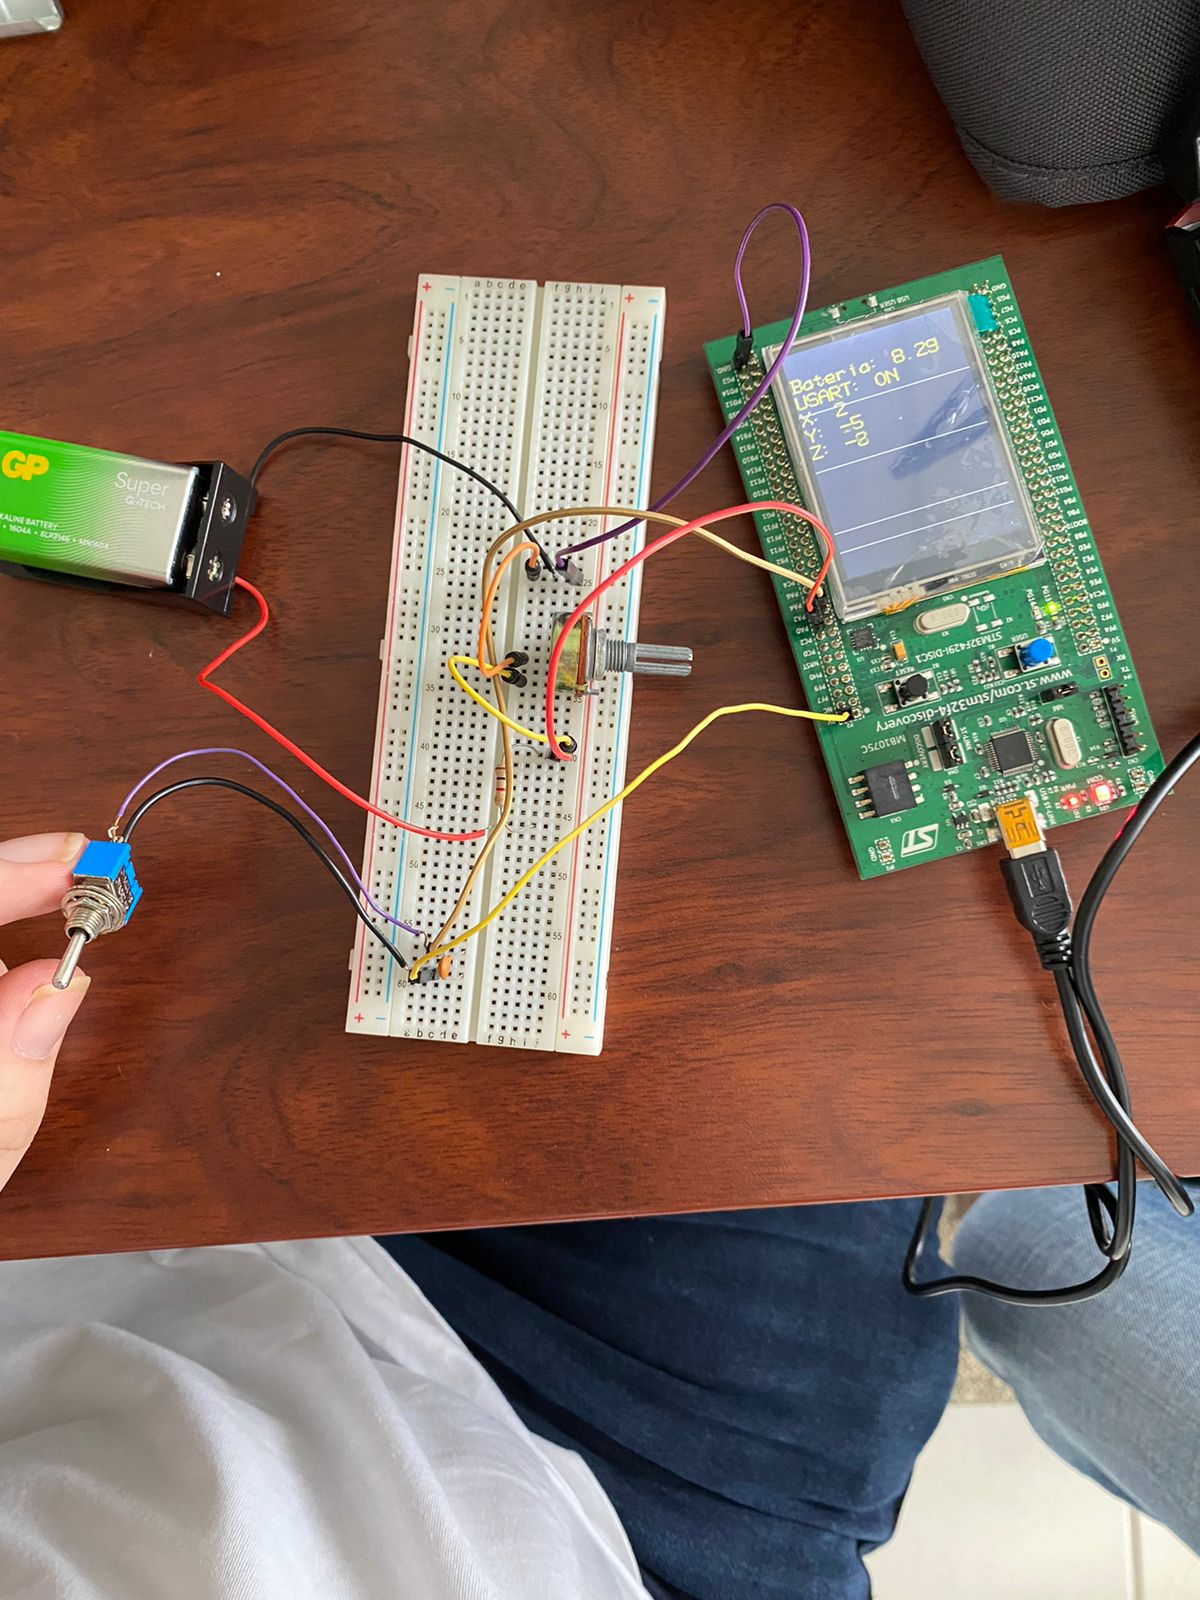
\includegraphics[width=\textwidth]{Imagenes/Prueba_USART2.jpg} 
    \caption{Prueba USART en estado ``ON''}
    \label{Fig:Prueba_USART2}
\end{subfigure}
\end{figure}

En las figuras \ref{Fig:Prueba_USART} y \ref{Fig:Prueba_USART2}, se observan las pruebas que se realizaron para verificar que cuando el switch se encuentra en ``OFF'', el microcontrolador lee que ese PIN esta en bajo, es decir, la comunicación USART esta desactiva como se observa en la pantalla LDC de la figura \ref{Fig:Prueba_USART}, cuando el switch esta en ``ON'', quiere decir que la el microcontrolador lee que el PIN se encuentra en alto y el LED verde del microcontrolador se enciende, es decir, que la comunicación USART se activa, como se observa en la pantalla LDC de la figura \ref{Fig:Prueba_USART2}. Para evitar el efecto rebote del switch, se le conectó un capacitor de 22 nF y no fue necesario conectarle una resistencia ya que este microcontrolador trae una resistencia interna según la hoja de datos \cite{stm32micro, datasheet}. 

\subsubsection{Verificación del funcionamiento de la Batería y el USART al mismo tiempo}

\begin{figure}[H]
    \begin{subfigure}{0.5\textwidth}
    \centering
    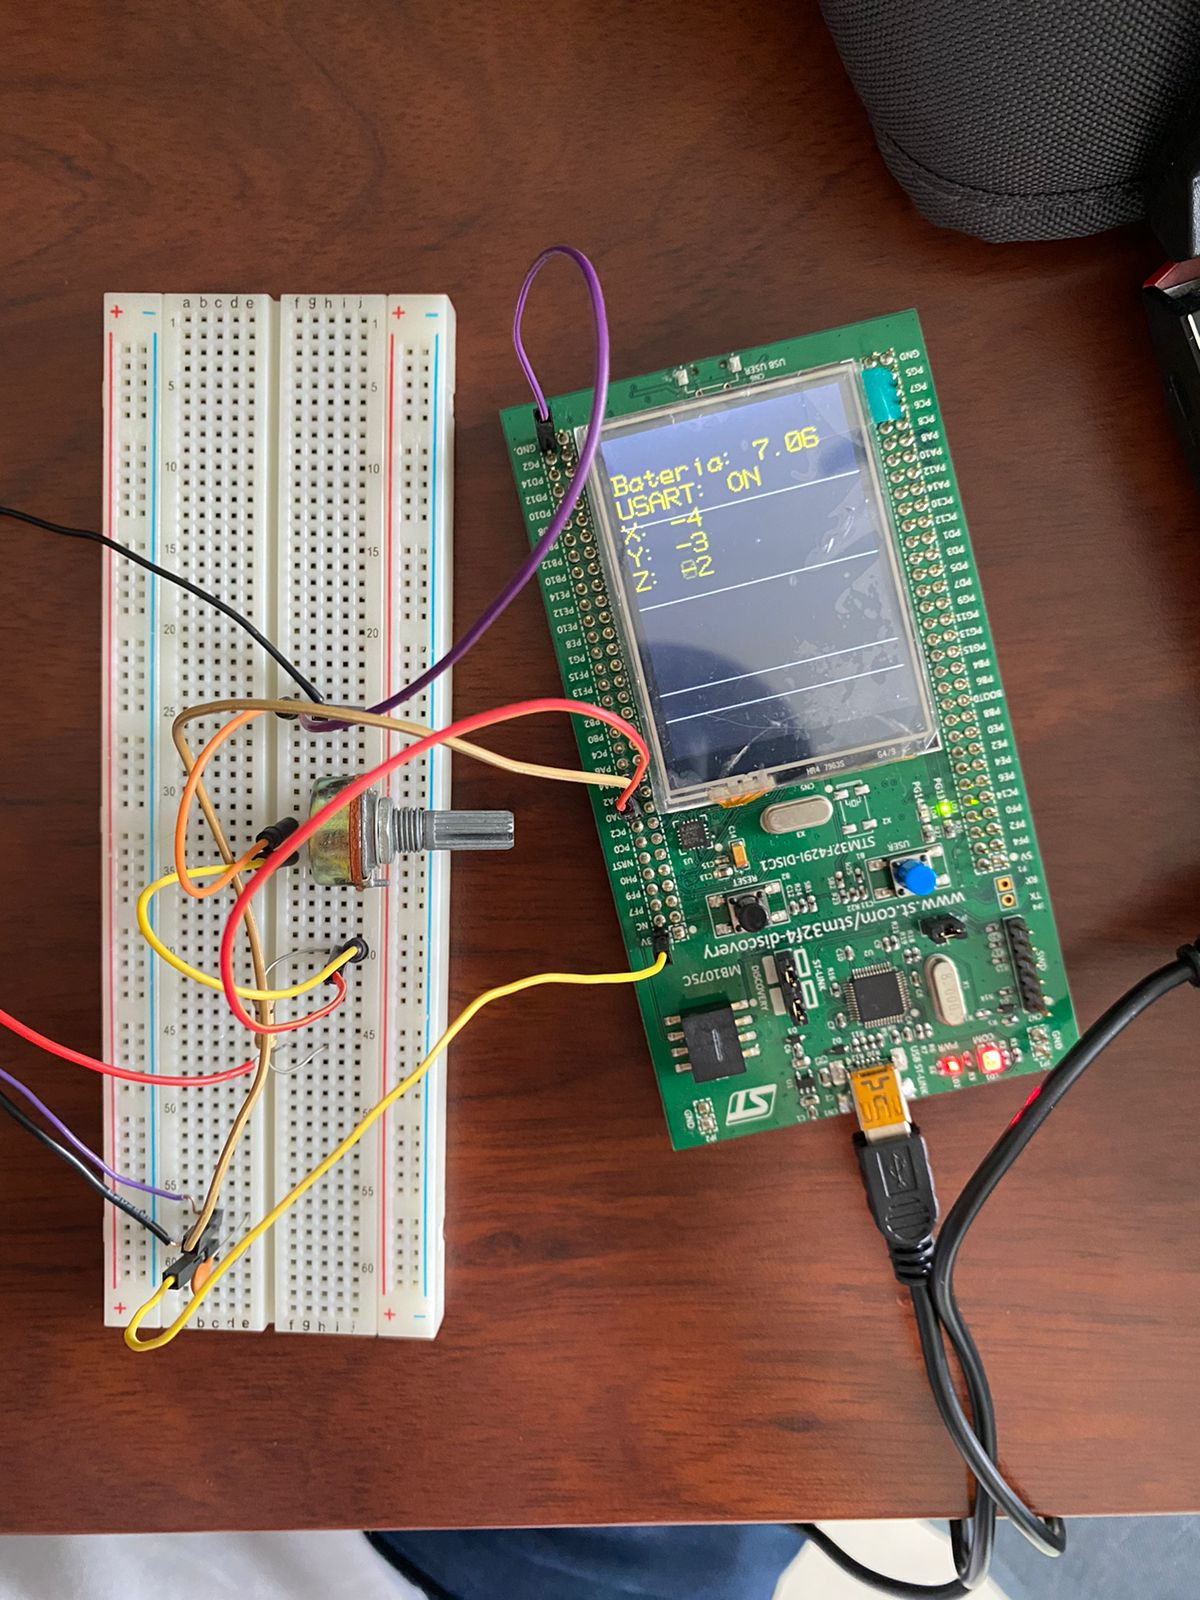
\includegraphics[width=0.9\textwidth]{Imagenes/Prueba_Bat_USART.jpg} 
    \caption{Prueba del funcionamiento de la USART y la Batería cercano a 7V.}
    \label{Fig:Prueba_Bat_USART}
\end{subfigure}
\begin{subfigure}{0.5\textwidth}
    \centering
    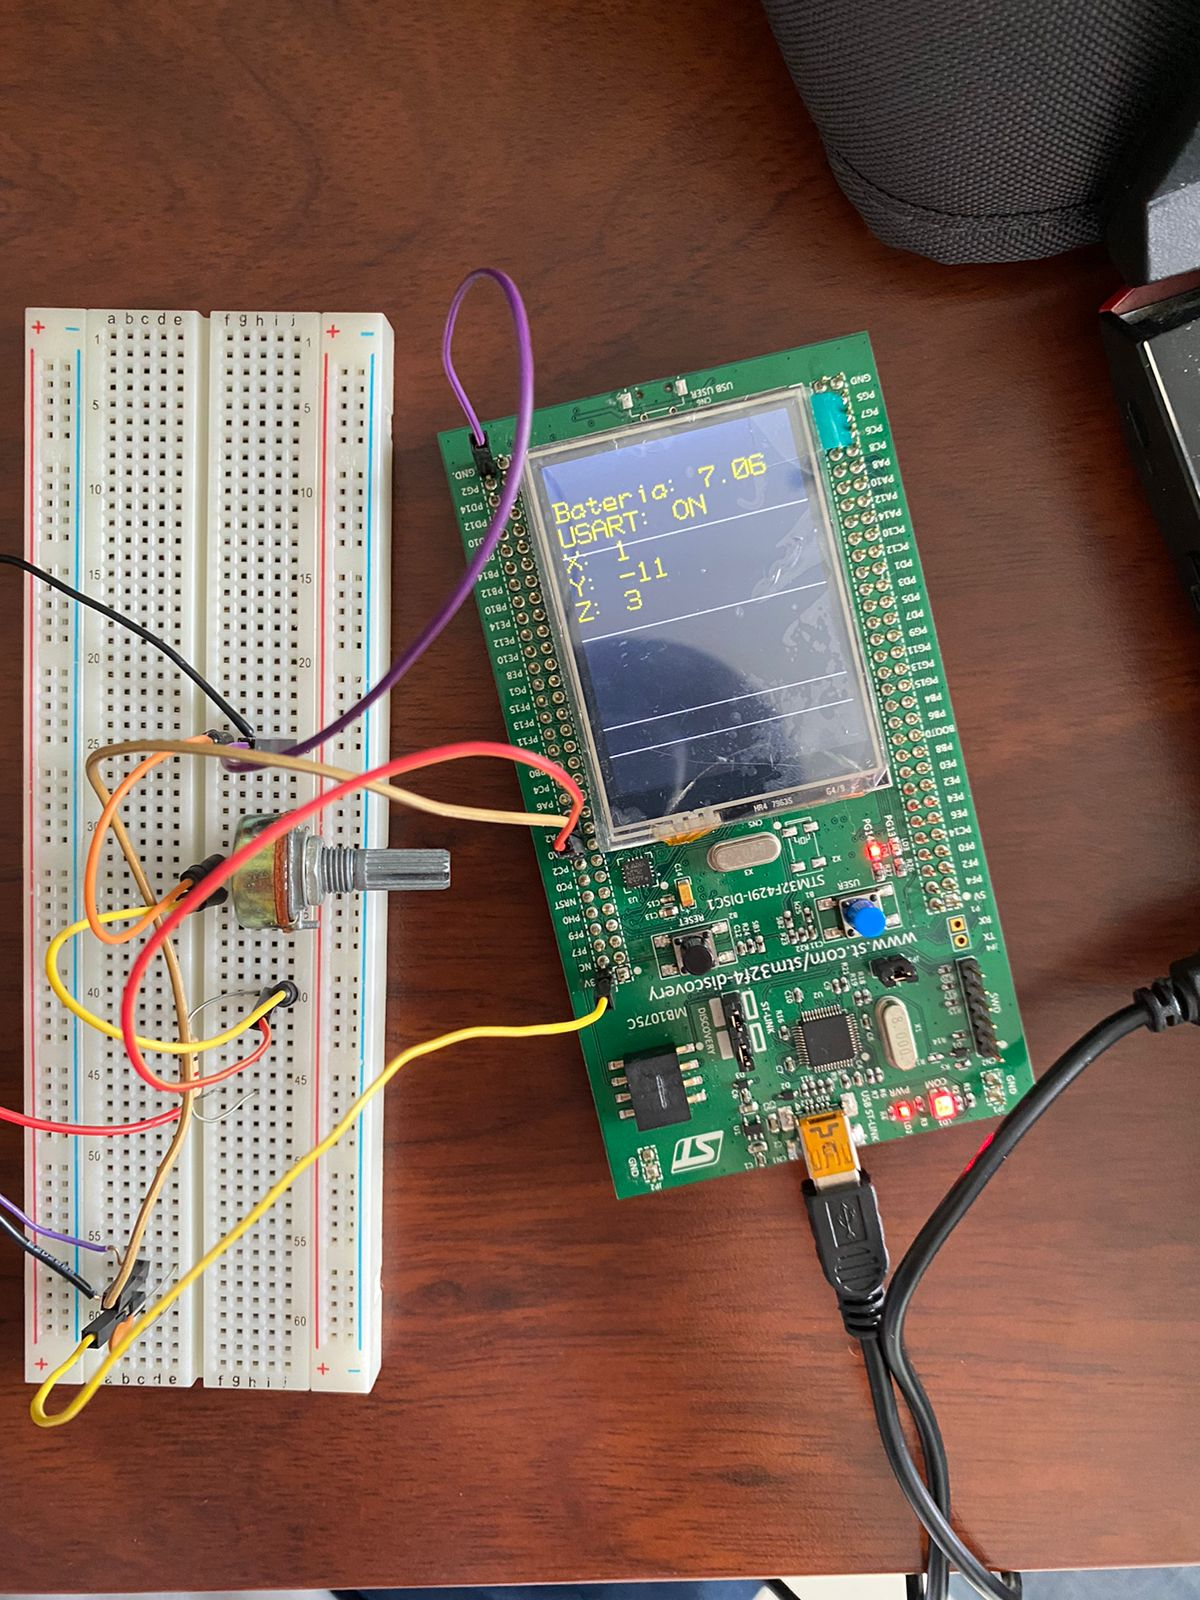
\includegraphics[width=\textwidth]{Imagenes/Prueba_Bat_USART2.jpg} 
    \caption{Prueba del funcionamiento de la USART y la Batería cercano a 7V.}
    \label{Fig:Prueba_Bat_USART2}
\end{subfigure}
\end{figure}

En las figuras \ref{Fig:Prueba_Bat_USART} y \ref{Fig:Prueba_Bat_USART2}, se observan como las 2 pruebas anteriores funcionan al mismo tiempo, cabe a destacar que las mangones que se muestran son únicamente cuando la tensión está cerca de la tensión de operación, es decir, esta cerca de los 7 V, de manera que el LED rojo se enciende y además se activa la comunicación USART, entonces los LED's parpadean de rojo a verde, comunicando que la comunicación USART esta activa y que la tensión de la batería esta cerca de la tensión de operación.



\subsection{Verificación que los datos se envíen correctamente por USART}
Ahora, se debe verificar que los datos se envíen correctamente por USART para ser mostrados en una terminal de la computadora. La figura \ref{usart-data-received} ilustra que sí se reciben los datos desde la placa de desarrollo y son mostrados correctamente en la terminal. En el video que se incluye en la entrega de este reporte, los videos \tt{demo\_usart\_off} ilustra que por más movimiento que se haga a la placa, éste no enviará los datos por USART ya que el USART está deshabilitado. En cambio, los videos \tt{demo\_usart\_iot\_on\_*} se muestra que cuando el USART está habilitado, los datos son enviados por comunicación serial y se reciben correctamente en la terminal.
\begin{figure}[H]
    \centering
    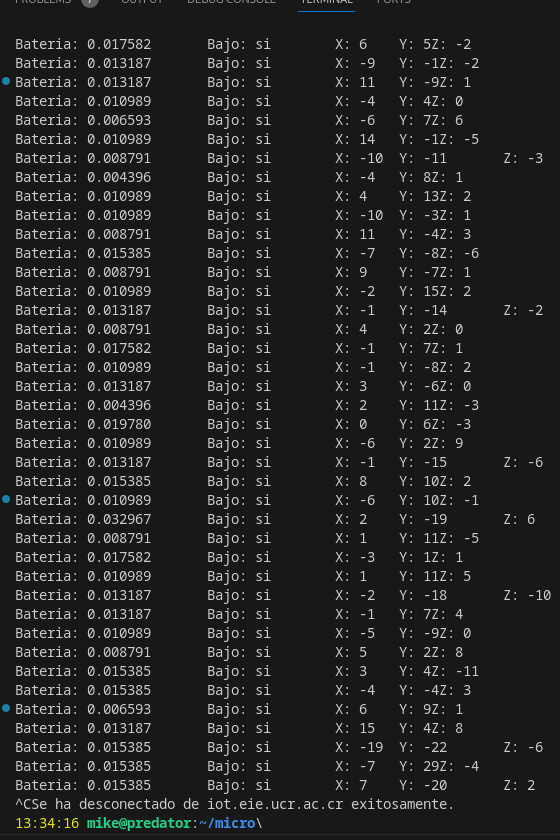
\includegraphics[width=12cm]{Imagenes/usart_data_received.png}
    \caption{Captura de pantalla de la terminal donde se reciben los datos por USART.}
    \label{usart-data-received}
\end{figure}

\subsection{Verificación de los datos se reflejen en iot.eie.ucr.ac.cr}
Luego, se debe comprobar que los datos recibidos por USART se envíen correctamente a \tt{iot.eie.ucr.ac.cr}. La figura \ref{iot-data-received} ilustra que los datos son enviados correctamente a Thingsboard y se muestran correctamente en el dashboard. Los videos \tt{demo\_usart\_iot\_on\_*} incluidos en la entrega ilustran que efectivamente los datos llegan correctamente a Thingsboard puesto que la página web se actualiza cuando se envía datos desde la placa de desarrollo.
\begin{figure}[H]
    \centering
    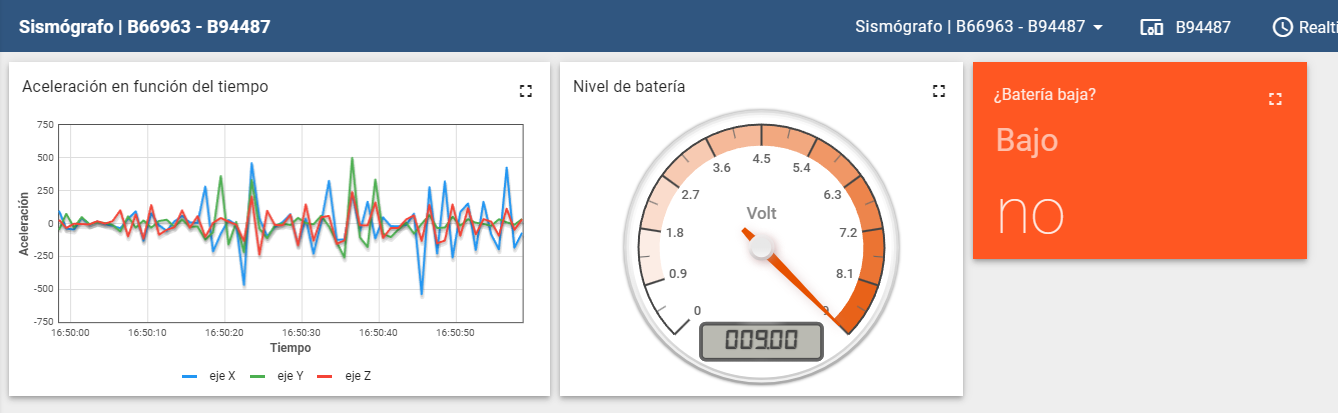
\includegraphics[width=\textwidth]{Imagenes/iot_data_received.png}
    \caption{Captura de pantalla de la terminal donde se envían a \tt{iot.eie.ucr.ac.cr} los datos.}
    \label{iot-data-received}
\end{figure}


\subsection{Verificación de las tensiones se encuentren dentro del rango seguro}

Con ayuda de un voltímetro se verificó que las tensiones que lee el microcontrolador se encuentran en rango seguro según la hoja del fabricante, y así evitar que se queme algún componente del microcontrolador \cite{stm32micro, datasheet}.


\begin{figure}[H]
    \begin{subfigure}{0.5\textwidth}
    \centering
    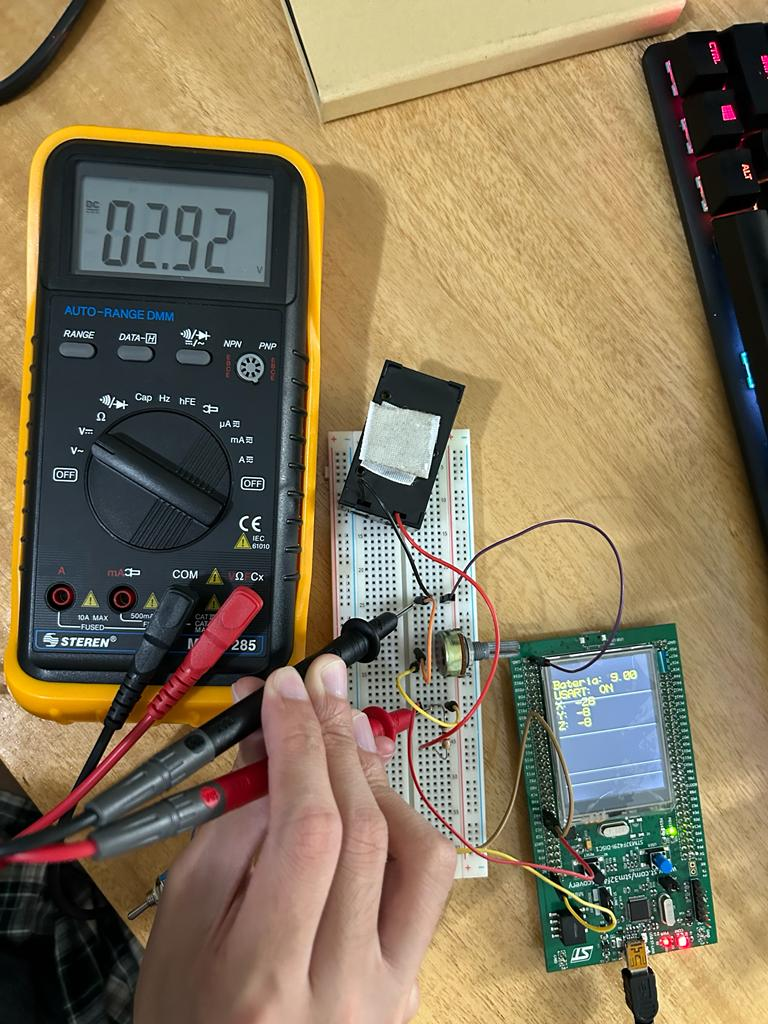
\includegraphics[width=\textwidth]{Imagenes/BATERIA.jpg} 
    \caption{Lectura de la tensión que lee del PIN PA0 (la batería) el microcontrolador}
    \label{Fig:BATERIA}
\end{subfigure}
\begin{subfigure}{0.5\textwidth}
    \centering
    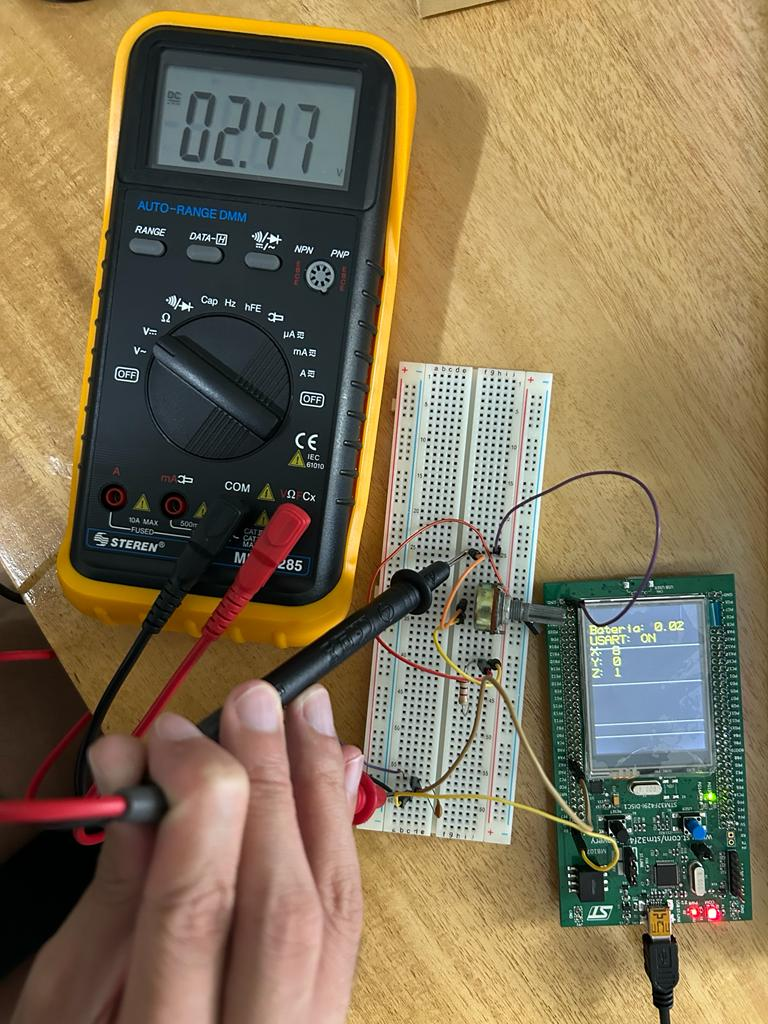
\includegraphics[width=\textwidth]{Imagenes/USART.jpg} 
    \caption{Lectura de la tensión que lee del PIN PA2 el microcontrolador}
    \label{Fig:USART}
\end{subfigure}
\end{figure}

Como se puede ver, en las figuras \ref{Fig:BATERIA} y \ref{Fig:USART} se observa que el voltaje que marca son 2.92V para la etapa de la batería y para la etapa del switch que controla el USART marca 2.47V, según la hoja del fabricante el valor máximo de tensión que soporta los pines es 4 V según la hoja del fabricante \cite{stm32micro, datasheet}, y ambos valores están por debajo de esa de esa tensión, por lo tanto se concluye que se está trabajando con unas tensiones seguras para el microcontrolador y así no dañar el STM32F429.




































